\section{FileSystem}
    \begin{figure}[h]
        \centering
        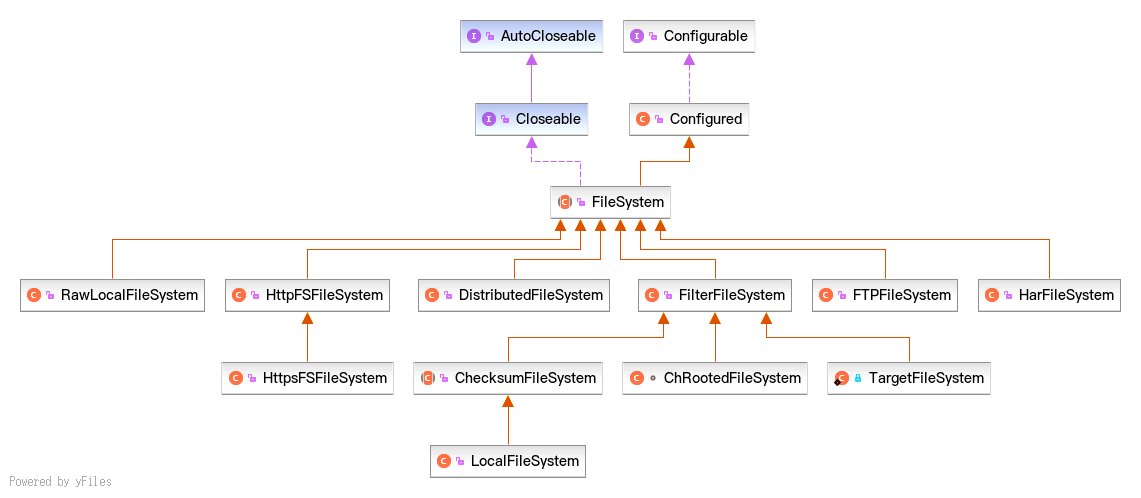
\includegraphics[width=1\linewidth]{filesystemclass}
        \caption{FileSystem 类的 UML 类图}
        \label{fig:filesystemclass}
    \end{figure}
\subsection{}
    FileSystem作为文件系统最顶层抽象类,描述了一个文件系统的抽象定义,继承了org.apache.hadoop.conf.Configured配置基类,并实现了java.io.Closeable接口。提供了从XML配置文件生成符合配置描述的文件系统的功能。\\
    FileSystem抽象类定义了文件系统所具有的基本特征和基本操作。FileSystem具有以下属性:
    \begin{java}[caption=FileSystem attribute]
public static final String FS_DEFAULT_NAME_KEY = 
    CommonConfigurationKeys.FS_DEFAULT_NAME_KEY;
public static final String DEFAULT_FS = 
    CommonConfigurationKeys.FS_DEFAULT_NAME_DEFAULT;

public static final Log LOG = LogFactory.getLog(FileSystem.class);

public static final int SHUTDOWN_HOOK_PRIORITY = 10;

public static final String TRASH_PREFIX = ".Trash";

static final Cache CACHE = new Cache();

private Cache.Key key;

private static final Map<Class<? extends FileSystem>, Statistics> 
    statisticsTable =
        new IdentityHashMap<Class<? extends FileSystem>, Statistics>();

protected Statistics statistics;

private Set<Path> deleteOnExit = new TreeSet<Path>();

    \end{java}
    其中Cache CACHE用于缓存已打开的,可缓存的文件系统,启用Cache可以直接复用已打开的文件系统而不必每次都从配置文件生成新的文件系统实例。\\
    Cache.Key key所包含的内容就是一个URI的信息及其用户名,作为Cache中Map的键,与Cache一同提供了通过一个合法的URI信息与用户名快速获取到缓存中存在的一个文件系统的对象,从而能够获取到指定文件系统中文件信息的功能。\\
    statisticsTable 主要用于保存文件系统的统计信息,作为其Value的Statistics类使用了java.util.concurrent.atomic包中的原子变量属性,提高统计信息的一致性,保证线程安全的原子读写操作的同时,提高了并行性能。\\
    deleteOnExit作为文件缓存,用来收集当前缓存中的文件Path。当文件系统关闭或JVM退出的时候,调用同步方法processDeleteOnExit将缓存中的文件全部安全删除。\\
    \\
    FileSystem为用户提供了一个访问不同文件系统的统一的接口,屏蔽了不同文件系统操作访问上的差异性。其主要提供的方法可以分为两大类:一部分是处理文件和目录相关的事务,另一部分则是文件的读写操作。\\
    以下是FileSystem中定义的12个抽象方法,这12个方法应该是一个文件系统应具有的基本操作,而具体的实现则是取决于不同具体的文件系统的特点。
    \begin{java}[caption=FileSystem abstract method]
public abstract URI getUri();

public abstract FSDataInputStream open(Path f, int bufferSize) throws IOException;

public abstract FSDataOutputStream create(Path f,
    FsPermission permission,
    boolean overwrite,
    int bufferSize,
    short replication,
    long blockSize,
    Progressable progress) throws IOException;

public abstract FSDataOutputStream append(Path f, int bufferSize, Progressable progress) throws IOException;

public abstract boolean rename(Path src, Path dst) throws IOException;

public abstract boolean delete(Path f) throws IOException;

public abstract boolean delete(Path f, boolean recursive) throws IOException;

public abstract FileStatus[] listStatus(Path f) throws IOException;

public abstract void setWorkingDirectory(Path new_dir);

public abstract Path getWorkingDirectory();

public abstract boolean mkdirs(Path f, FsPermission permission) throws IOException;

public abstract FileStatus getFileStatus(Path f) throws IOException;

    \end{java}

\subsection{基于FileSystem实现的文件系统概述}
    \subsubsection{RawLocalFileSystem}
        RawLocalFileSystem是hadoop中实现的本地文件系统,在该类中与文件元数据和目录相关的操作,都是通过装饰器模式适配到java.io.File的对应API来完成的。\\
        LocalFSFileInputStream的构造函数如下:
        \begin{java}[caption=LocalFSFileInputStream]
class LocalFSFileInputStream extends FSInputStream {
    public LocalFSFileInputStream(Path f) throws IOException {
        this.fis = new TrackingFileInputStream(pathToFile(f));
    }
}
        \end{java}
        \begin{java}[caption=TrackingFileInputStream]
class TrackingFileInputStream extends FileInputStream {
    public TrackingFileInputStream(File f) throws IOException {
        super(f);
    }
}
\end{java}

    \subsubsection{FilterFileSystem}
        FilterFileSystem类主要是在其内部定义了一个Filesystem属性用于包含其他文件系统,FilterFileSystem用作其基本文件系统,可能性的提供转换数据或附加功能。\\
        FilterFileSystem类本身简单地覆盖FileSystem的所有方法,将所有请求传递给其包含的文件系统。
        \begin{java}[caption=FilterFileSystem]
public class FilterFileSystem extends FileSystem {
    protected FileSystem fs;
    @Override
    public void concat(Path f, Path[] psrcs) throws IOException {
        fs.concat(f, psrcs);
    }
}
        \end{java}

    \subsubsection{ChecksumFileSystem}
        ChecksumFileSystem类是一个基于校验和的文件系统的抽象类,它继承自FilterFileSystem类,其特点就是在客户端为每一个原生文件(raw file)创建一个扩展名为“.crc”的校验和文件,用来校验原生文件的完整性。
        \begin{java}[caption=ChecksumFileSystem]
private int bytesPerChecksum = 512; 
private boolean verifyChecksum = true; 
        \end{java}
        
        ChecksumFSInputChecker用于在写入过程中根据配置生成其校验和文件,ChecksumFSOutputSummer用于读取过程中依据校验文件对原生文件进行正确性校验。
        \begin{itemize}
            \item[*] org.apache.hadoop.fs.ChecksumFileSystem.ChecksumFSInputChecker      
            \item[*] org.apache.hadoop.fs.ChecksumFileSystem.ChecksumFSOutputSummer
        \end{itemize}

    \subsubsection{LocalFileSystem}
        LocalFileSystem类实现了FileSystem的API,它是一个基于校验和的本地文件系统。\\
        它是以RawLocalFileSystem为基本文件系统。
        \begin{java}[caption=LocalFileSystem]
public LocalFileSystem() {  
    this(new RawLocalFileSystem());  
}  
public LocalFileSystem(FileSystem rawLocalFileSystem) {  
    super(rawLocalFileSystem);  
    rfs = rawLocalFileSystem;  
} 
        \end{java}
        
        reportChecksumFailure方法实现了向文件系统报告校验和文件出错,同时把出错的校验和文件重命名后,移动到指定的bad\_files目录中,在该目录中的文件是不能够被重新使用的。\\
        \begin{java}[caption=reportChecksumFailure]
public boolean reportChecksumFailure(Path p, FSDataInputStream in, long inPos, FSDataInputStream sums, long sumsPos) {
    try {
        File f = ((RawLocalFileSystem)fs).pathToFile(p).getCanonicalFile();
        String device = new DF(f, getConf()).getMount();
        File parent = f.getParentFile();
        File dir = null;
        while (parent != null && FileUtil.canWrite(parent) && parent.toString().startsWith(device)) {
            dir = parent;
            parent = parent.getParentFile();
        }

        if (dir==null) {
            throw new IOException("not able to find the highest writable parent dir");
        }
            
        File badDir = new File(dir, "bad_files");
        if (!badDir.mkdirs()) {
            if (!badDir.isDirectory()) {
            throw new IOException("Mkdirs failed to create " + badDir.toString());
            }
        }
        String suffix = "." + rand.nextInt();
        File badFile = new File(badDir, f.getName()+suffix);
        LOG.warn("Moving bad file " + f + " to " + badFile);
        in.close();                               // close it first
        boolean b = f.renameTo(badFile);                      // rename it
        if (!b) {
            LOG.warn("Ignoring failure of renameTo");
        }

        File checkFile = ((RawLocalFileSystem)fs).pathToFile(getChecksumFile(p));
        sums.close();
        b = checkFile.renameTo(new File(badDir, checkFile.getName()+suffix));
        if (!b) {
            LOG.warn("Ignoring failure of renameTo");
            }
    } catch (IOException e) {
        LOG.warn("Error moving bad file " + p + ": " + e);
    }
    return false;
}
        \end{java}

    \subsubsection{DistributedFileSystem}
        对HDFS的用户来说,DistributedFileSystem就代表了Hadoop分布式文件系统,用户只要操作DistributedFileSystem的对象来进行文件目录的建立、数据的存取操作,其他的都由DistributedFileSystem来完成,所以它为我们提供了一个HDFS的界面。
        \begin{java}[caption=DistributedFileSystem]
public class DistributedFileSystem extends FileSystem {  
    private Path workingDir;  
    private URI uri;  
    DFSClient dfs;  
    private boolean verifyChecksum = true;  
        
    static{  
        Configuration.addDefaultResource("hdfs-default.xml");  
        Configuration.addDefaultResource("hdfs-site.xml");  
    }  
    
    public DistributedFileSystem() {  
    }  
}  
        \end{java}

        但是在HDFS内部,通过适配器模式将真正的操作步骤是交给了与服务器端交互的HDFS客户端(DFSClient)去完成,实现与HDFS集群上的其他节点进行交互功能。
        \begin{java}[caption=DistributedFileSystem.rename]
public void rename(Path src, Path dst, final Options.Rename... options) throws IOException {
    statistics.incrementWriteOps(1);
    storageStatistics.incrementOpCounter(OpType.RENAME);
    final Path absSrc = fixRelativePart(src);
    final Path absDst = fixRelativePart(dst);
    try {
        dfs.rename(getPathName(absSrc), getPathName(absDst), options);
    } catch (UnresolvedLinkException e) {
        final Path source = getFileLinkStatus(absSrc).getPath();
        new FileSystemLinkResolver<Void>() {
            @Override
            public Void doCall(final Path p) throws IOException {
                dfs.rename(getPathName(source), getPathName(p), options);
                return null;
            }
            @Override
            public Void next(final FileSystem fs, final Path p) throws IOException {
                return doCall(p);
            }
        }.resolve(this, absDst);
    }
}
        \end{java}
        \begin{figure}[h]
            \centering
            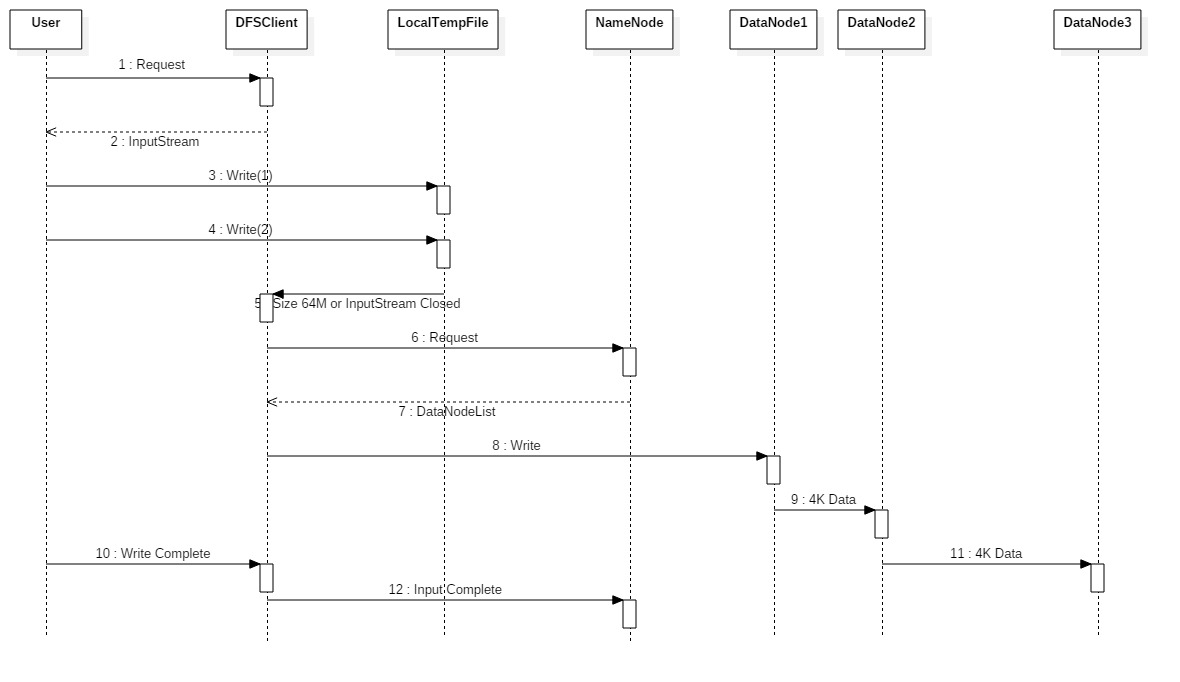
\includegraphics[width=1\linewidth]{HDFSInputTime}
            \caption{一个简单的HDFS写入操作时序图}
            \label{fig:HDFS Input Time}
        \end{figure}


    \subsubsection{其他文件系统实现}
        \begin{itemize}
            \item[*] HarFileSystem
            \item[*] HttpFSFileSystem
            \item[*] HttpsFSFileSystem
            \item[*] FTPFileSystem
        \end{itemize}


%% 结束
\endinput